\documentclass{article}
\usepackage[utf8]{inputenc}
\usepackage{tikz}
\usetikzlibrary{positioning}
\usetikzlibrary{shapes}

\begin{document}

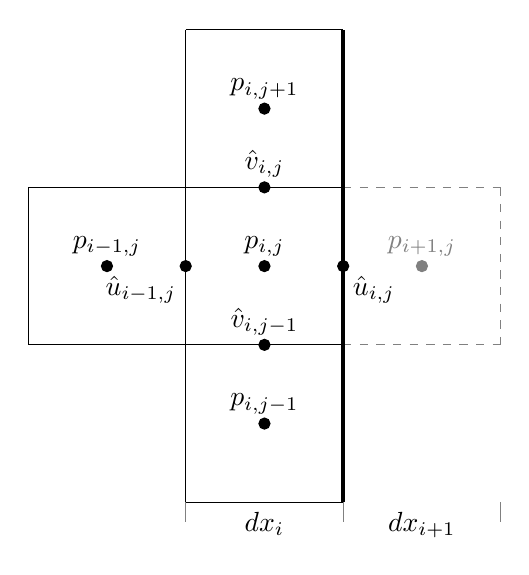
\begin{tikzpicture}
%grid
%horizontal
\draw[black, thin] (-1,3) -- (1,3);
\draw[black, thin] (1,1) -- (-3,1);
\draw[black, thin] (1,-1) -- (-3,-1);
\draw[gray, thin, dashed] (1,1) -- (3,1);
\draw[gray, thin, dashed] (1,-1) -- (3,-1);
\draw[black, thin] (-1,-3) -- (1,-3);

%vertical
\draw[black, thin] (-3,1) -- (-3,-1);
\draw[black, thin] (-1,3) -- (-1,-3);
\draw[black, ultra thick] (1,-3) -- (1,3);
\draw[gray, thin, dashed] (3,1) -- (3,-1);
%nodes
\filldraw [black] (0,0) circle (2pt) node[anchor=south] {$p_{i,j}$};
\filldraw [black] (0,2) circle (2pt) node[anchor=south] {$p_{i,j+1}$};
\filldraw [gray] (2,0) circle (2pt) node[anchor=south] {$p_{i+1,j}$};
\filldraw [black] (0,-2) circle (2pt) node[anchor=south] {$p_{i,j-1}$};
\filldraw [black] (-2,0) circle (2pt) node[anchor=south] {$p_{i-1,j}$};

\filldraw [black] (1,0) circle (2pt) node[anchor=north west] {$\hat{u}_{i,j}$};
\filldraw [black] (-1,0) circle (2pt) node[anchor=north east] {$\hat{u}_{i-1,j}$};
\filldraw [black] (0,1) circle (2pt) node[anchor=south] {$\hat{v}_{i,j}$};
\filldraw [black] (0,-1) circle (2pt) node[anchor=south] {$\hat{v}_{i,j-1}$};
%dx dy anchors
\node[black, thin, anchor=north](dxi) at (0,-3){$dx_i$};
\node[black, thin, anchor=north](dxip) at (2,-3){$dx_{i+1}$};
\draw[gray, thin] (-1,-3) -- (-1,-3.25);
\draw[gray, thin] (1,-3) -- (1,-3.25);
\draw[gray, thin] (3,-3) -- (3,-3.25);

\end{tikzpicture}
\end{document}
